% !TeX program = xelatex
% !TeX encoding = UTF-8 Unicode
% !BIB program = biber

% !TeX root = document.tex
% !TeX encoding = UTF-8 Unicode

\documentclass[sumario=tradicional,
	12pt,
	openright,
	twoside,
	a4paper,
	english,
	french,
	brazil]{abntex2}

% Set font in LuaLaTeX and XeLaTeX. Does not work in PDFLaTeX
\usepackage{fontspec}
\defaultfontfeatures{Ligatures=TeX,Scale=MatchLowercase}
\renewcommand{\baselinestretch}{1.5} % Line height of 1.5

% Basics packages
\usepackage[brazil]{babel}
\usepackage[useregional]{datetime2}
\usepackage[style=abnt]{biblatex}
\usepackage[decimalsymbol=comma,
	input-complex-roots=j,
	output-complex-root=j,
	complex-root-position=after-number,
	loctolang={BR:portuguese,UK:english}]{siunitx} % SI units
%\edef\pdfcreationdate {\pdffeedback creationdate} % fixes datetime import in LuaLaTeX and XeLaTeX
\usepackage[top=3cm,bottom=2cm,left=3cm,right=2cm]{geometry}

% Image manipulation
\usepackage{graphicx} % For images
\usepackage{rotate} % To rotate images
\usepackage[section]{placeins} % Prevents figures from floating to wrong places
\usepackage{epsf}
\usepackage{caption}[2004/07/16]

% Math related
\usepackage{amssymb}
\usepackage{amsmath} % Mathematic symbols and stuff
\usepackage{amsfonts} % Mathematical fonts
\usepackage{cancel} % In math mode, variables to strike
\usepackage{subscript} % For subscript

% Table manipulation
\usepackage{longtable} % For long tables that take more than one page
\usepackage{multirow} % Multirow tables
\usepackage{tabulary} % Table tabulation
% Makes the column type L, that is centered and allows line wrap.
\usepackage{array}
\newcolumntype{L}{>{\centering\arraybackslash}m{3cm}}

% Utilities
\usepackage[section]{minted} % Code highlighting with Pygments
% \usepackage[usenames,dvipsnames]{xcolor} % More colors:
\usepackage{pdfpages} % Advanced PDF importing
\usepackage{pdflscape} % One page panorama
\usepackage[european,cuteinductors,smartlabels]{circuitikz} % For circuits
\usepackage{indentfirst} % Indents first paragraph after section
\usepackage{chngcntr} % Change numberings
\usepackage{csquotes} % \enquote
\usepackage{url}
\usepackage{ragged2e} % Justify
\usepackage{lastpage}
%\usepackage{fancyhdr} % Set headers and footers
\usepackage[Lenny]{fncychap} % Square chapter
\usepackage{acro} % abbreviations and accronyms

\usetikzlibrary{shapes,arrows}

\renewcommand{\rm}{\textrm} % needed with memoir
\renewcommand{\chaptermark}[1]{\markboth{\chaptername\ \thechapter. \ #1}{ }}
\renewcommand{\sectionmark}[1]{\markright{\thesection. \ #1}}
\renewcommand{\tocheadstart}{\rm}
\renewcommand{\ABNTEXchapterfont}{\rm}
\renewcommand{\ABNTEXchapterfontsize}{\huge}
\ChTitleVar{\ABNTEXchapterfontsize\ABNTEXchapterfont}
\setsecheadstyle{\bfseries\Large}

% Removes red boxes when lexer can't understand something (like @ in Python 3)
\AtBeginEnvironment{minted}{\renewcommand{\fcolorbox}[4][]{#4}}

% pythoncode environment for hightlight
\newminted{python3}
{autogobble,linenos,python3,fontseries=Consolas,fontsize=\scriptsize,frame=lines}
\newmintedfile[python]{python3}
{autogobble,linenos,python3,fontseries=Consolas,fontsize=\scriptsize,frame=lines}

% ccode environment for highlight
\newminted{c}
{autogobble,linenos,fontseries=Consolas,fontsize=\scriptsize,frame=lines}

\newcommand{\norm}[1]{\left\lVert#1\right\rVert}

% !TeX root = document.tex
% !TeX encoding = UTF-8 Unicode

%%criar um novo estilo de cabeçalhos e rodapés
\makepagestyle{cefet}
  %%cabeçalhos
  \makeevenhead{cefet} %%pagina par
     {~}
     {~}
     {\rightmark}
  \makeoddhead{cefet} %%pagina ímpar ou com oneside
     {~}
     {~}
     {\rightmark}
  \makeheadrule{cefet}{\textwidth}{\normalrulethickness} %linha
  %% rodapé
  \makeevenfoot{cefet}
     {~} %%pagina par
     {\thepage}
     {~} 
  \makeoddfoot{cefet} %%pagina ímpar ou com oneside
     {~}
     {\thepage}
     {~}

\makepagestyle{cefetchapter}
  %%cabeçalhos
  \makeevenhead{cefetchapter} %%pagina par
     {~}
     {~}
     {~}
  \makeoddhead{cefetchapter} %%pagina ímpar ou com oneside
     {~}
     {~}
     {~}
  %% rodapé
  \makeevenfoot{cefetchapter}
     {~} %%pagina par
     {\thepage}
     {~} 
  \makeoddfoot{cefetchapter} %%pagina ímpar ou com oneside
     {~}
     {\thepage}
     {~}

% !TeX root = document.tex
% !TeX encoding = UTF-8 Unicode

% probably a good idea for the nomenclature entries:
\acsetup{first-style=short}

\DeclareAcronym{LPV}{
    short = LPV,
    long  = {Variação linear de parâmetros, do inglês \textit{Linear Parameter Varying}},
    class = abbrev
}

\DeclareAcronym{MPC}{
    short = MPC,
    long  = {Controle preditivo por modelo, do inglês \textit{Model Predictive Control}},
    class = abbrev
}

\DeclareAcronym{DMPC}{
    short = DMPC,
    long  = {Controle preditivo por modelo discreto, do inglês \textit{Discrete Model Predictive Control}},
    class = abbrev
}

\DeclareAcronym{SPD}{
    short = SPD,
    long  = Sistema a Parâmetros Distribuídos,
    class = abbrev
}

\DeclareAcronym{SPC}{
    short = SPC,
    long  = Sistema a Parâmetros Concentrados,
    class = abbrev
}

\DeclareAcronym{DMC}{
    short = DMC,
    long  = {Controle Dinâmico por Matriz, do inglês \textit{Dynamic Matrix Control}},
    class = abbrev
}

\DeclareAcronym{IMC}{
    short = IMC,
    long  = {Controle por Modelo Interno, do inglês \textit{Internal Model Control}},
    class = abbrev
}

\DeclareAcronym{EDP}{
    short = EDP,
    long  = Equação Diferencial Parcial,
    class = abbrev
}

\DeclareAcronym{ARMAX}{
    short = ARMAX,
    long  = {Modelo autoregressivo de média variável com entradas exógenas, do inglês \textit{Autoregressive–moving-average with exogenous inputs model}},
    class = abbrev
}

\DeclareAcronym{AT}{
    short = \(A'\),
    long  = Transposta de uma matriz,
    sort  = A',
    class = nomencl
}


\selectlanguage{brazil}
\addbibresource{bibliothek.bib}
\hypersetup{
  unicode    = true,
  pdftitle   = {Implementação de controlador MPC em um sistema a parâmetros distribuídos via subsistemas interconectados},
  pdfsubject = {Implementação de controlador MPC em um sistema a parâmetros distribuídos via subsistemas interconectados},
  pdfauthor  = {Álan Crístoffer e Sousa}
}

\begin{document}
  \selectlanguage{brazil}
  \pretextual{}
  \renewcommand{\printtoctitle}{\chapter*}
  \renewcommand{\printloftitle}{\chapter*}
  \renewcommand{\printlottitle}{\chapter*}

  \textual{}
  \pagestyle{cefetchapter}
  \pagenumbering{roman}
  % !TeX root = document.tex
% !TeX encoding = UTF-8 Unicode

%================================================================================================
%=========================================== CAPA 1 =============================================
%================================================================================================

\vspace*{1.0cm}

\begin{center}
    {\textsc  Centro Federal de Educaçào Tecnológica de Minas Gerais\\
        \textit{Campus} Divinópolis\\
        Graduação em Engenharia Mecatrônica}
\end{center}

\vspace*{3.0cm}

\begin{center}
    \large Álan Crístoffer e Sousa
\end{center}

\vspace*{2.5cm}

\begin{center}
    \Large{\textsc{Implementação de controlador MPC em um sistema a parâmetros
                  distribuídos via subsistemas interconectados}} % alterar
                  % também mais abaixo.
\end{center}

\vspace*{4cm}

\epsfxsize=0.175\columnwidth{}
\centerline{\epsffile{imgs/cefet.eps}}

\null\vfill

\begin{center}
    Divinópolis\\
    \(2018\) % alterar também mais abaixo.
\end{center}

\thispagestyle{empty}
\cleardoublepage{}

%================================================================================================
%=========================================== CAPA 2 =============================================
%================================================================================================

\vspace*{1cm}

\begin{center}
    \large Álan Crístoffer e Sousa
\end{center}

\vspace*{1.5cm}

\begin{center}
    \Large{\textsc{Implementação de controlador MPC em um sistema a parâmetros
                  distribuídos via subsistemas interconectados}} % alterar
                  % também mais acima.
\end{center}

\vspace*{1.5cm}

\begin{flushright}
    \begin{minipage}{9.0cm}
        Monografia de Trabalho de Conclusão de Curso apresentada ao Colegiado de
        Graduação em Engenharia Mecatrônica como  parte dos requisitos exigidos
        para a obtenção do título de Engenhario Mecatrônico.\\
        Eixo de Formação: Modelagem e Controle de Processos.

        \vspace*{1cm}

        Orientador: Prof.\ Dr.\ Valter Júnior de Souza Leite\\
        Coorientador: Prof.\ Dr.\ Ignacio Rubio Scola
    \end{minipage}
\end{flushright}

\vspace*{1cm}

\epsfxsize=0.175\columnwidth{}
\centerline{\epsffile{imgs/cefet.eps}} % Aqui poderia ser substituido por um logo do curso ou do campus

\null\vfill

\begin{center}
    Divinópolis\\
    \(2018\) % alterar também mais acima.
\end{center}

\cleardoublepage{}

%================================================================================================
%============================== Ficha (Somente na versão final) =================================
%================================================================================================

%\epsfxsize=0.925\columnwidth
%\epsffile{ficha.ps} % após scanear, colocar a ficha catalográfica do texto
\cleardoublepage{}

%================================================================================================
%============================== Folha de aprovação (Somente na versão final) ====================
%================================================================================================

%\epsfxsize=0.925\columnwidth
%\epsffile{folha.ps} % após scanear, colocar a folha de aprovação do texto
\cleardoublepage{}

  % !TeX root = document.tex
% !TeX encoding = UTF-8 Unicode

%======================================== Dedicatória =========================================
\null{}
\vfill{}
\begin{flushright}
    \begin{minipage}{6.5cm}
        \textsc{A minha família, que sempre me apoiou nessa caminhada.}
    \end{minipage}\\[8mm]
\end{flushright}

\cleardoublepage{}
%==============================================================================================

  % !TeX root = document.tex
% !TeX encoding = UTF-8 Unicode

%======================================= Agradecimentos =======================================
\chapter*{Agradecimentos}

\noindent Agradeço,\\[2mm]
ao Prof.\@Pedro os cinco anos de valorosa orientação e a oportunidade de chegar
até Campinas, onde finalmente pude encontrar o meu verdadeiro caminho.\\[2mm]
aos colegas de trabalho mais próximos: Giórgio, Renato, Vinícius e Valter a
convivência descontraída e as trocas de experiências.\\[2mm]
aos demais colegas do Departamento de Telemática a ótima convivência.\\[2mm]
aos professores da FEEC:\@Ivanil, Paulo Valente, Von Zuben, Ivan Ricarte e
Geromel, os ótimos cursos oferecidos.\\[2mm]
aos professores Maurício C. de Oliveira (UCSD-EUA) e Pierre-Alexandre Bliman
(INRIA-França) pelas parcerias e discussões frutíferas.\\[2mm]
aos membros da banca examinadora os comentários, sugestões e contribuições, que
ajudaram a melhorar a qualidade e a redação final do manuscrito.\\[2mm]
À agência FAPESP o apoio financeiro concedido durante todo o período de
doutoramento.\\[2mm]
À FEEC/UNICAMP a ótima estrutura que oferece aos estudantes e
pesquisadores.\\[2mm]
À CAPES o portal de periódicos eletrônicos, que permite o acesso rápido e
eficiente ao conhecimento científico.\\[2mm]
ao Google o complemento que faz ao item anterior.\\[2mm]
a todos que de alguma forma contribu�ram com o meu progresso como aluno e como
Ser.

\thispagestyle{plain}
\cleardoublepage{}
%==============================================================================================

  % !TeX root = document.tex
% !TeX encoding = UTF-8 Unicode

%======================================== Frase Miss Brasil ===================================
\null{}
\vfill{}
\begin{flushright}
    \begin{minipage}{9.0cm}
        Não há nada como um sonho para criar o futuro.
    \end{minipage}
\end{flushright}

\begin{flushright}
    Victor Hugo
\end{flushright}

\cleardoublepage{}
%==============================================================================================

  % !TeX root = document.tex
% !TeX encoding = UTF-8 Unicode

\chapter*{Resumo}

\begin{abstract}
    Observadores permitem que o estado do sistema seja estimado dada sua saída.
    Sistemas a parâmetros distribuídos (\ac{SPD}) podem ser utilizados com
    observadores para recuperar informações ao longo do processo. Assim pode-se,
    por exemplo, medir-se a temperatura na extremidade de um sólido e, através
    desta, recuperar-se a temperatura em algum ponto no meio do sólido. Controle
    preditivo baseado em modelo (\ac{MPC} --- \textit{model predictive control})
    é uma técnica avançada de controle que lida com restrições. Ela já está
    estabelecida em indústrias que lidam com processos multi-variáveis de
    dinâmica lenta, especialmente na indústria petro-química. Ao combinar as
    duas técnicas é possível não apenas controlar uma variável em um ponto
    diferente daquele sendo medida, como também usar esta como uma restrição
    física no controle de outro ponto. Isto permite o controle de variáveis que
    são difíceis ou inviáveis de serem medidas diretamente. Embora ambas
    técnicas sejam bem discutidas isoladamente, há poucos artigos onde as duas
    são usadas em conjunto, o que sugere a existência de um campo a ser
    explorado. Assim propõe-se o desenvolvimento e a implementação de um
    controlador \ac{MPC} que utilize \ac{SPD} para realizar o controle de uma
    variável estimada em um ponto intermediário. Para isso será utilizada a
    planta presente no laboratório de sinais e sistemas. O modelo \ac{SPD}
    utilizado será o desenvolvido por~\textcite{masterthesis:nelson}. A
    implementação será feita utilizando os softwares \textit{Moirai} e
    \textit{Lachesis}, desenvolvidos \textit{in loco}, o que irá requerer
    modificações nos mesmos para funcionarem com as especificidades da planta.
    Também será feita alteração na microeletrônica da planta, com a finalidade
    de prover um meio alternativo para acionamento do forno. As modificações de
    hardware e software, em conjunto, permitirão maior flexibilidade no uso da
    planta, além de maior facilidade de uso. Pretende-se com este trabalho, que
    envolve principalmente as áreas de controle e computação, aprofundar os
    estudos do grupo de modelagem e controle de processos em \ac{SPD} com a
    metodologia de controle proposta, bem como facilitar futuros trabalhos na
    planta utilizada através do melhor desenvolvimento e teste da plataforma de
    controle.
\end{abstract}

Palavras-chave: Controle preditivo por modelo, sistema a parâmetros
                distribuídos, observador de Kalman


  \pdfbookmark[0]{\contentsname}{toc}
  \tableofcontents*{}
  \thispagestyle{plain}
  \cleardoublepage{}

  \renewcommand{\listfigurename}{Lista de figuras}
  \listoffigures*{}
  \thispagestyle{plain}
  \cleardoublepage{}

  \listoftables*{}
  \thispagestyle{plain}
  \cleardoublepage{}

  \listofcodes*{}
  \thispagestyle{plain}
  \cleardoublepage{}

  % !TeX root = document.tex
% !TeX encoding = UTF-8 Unicode

\chapter*{Lista de acrônimos e notações}

\printacronyms[include-classes=abbrev,name=]
\printacronyms[include-classes=nomencl,name=]

\thispagestyle{plain}

  \cleardoublepage{}

  \pagenumbering{arabic}
  \pagestyle{cefet}
  \aliaspagestyle{chapter}{cefetchapter}

  \newtheorem{theorem}{Teorema}
  
  \counterwithin{figure}{chapter}
  \counterwithin{table}{chapter}
  
  % !TeX root = document.tex
% !TeX encoding = UTF-8 Unicode

\chapter*{Introdução e Contextualização}%
\label{introducao}

MPC é uma técnica de controle avançada que utiliza o modelo do sistema para
prever a saída em momentos futuros e, com isso, gerar uma estratégia de
controle. Para isso é utilizado o conceito de controle por horizonte recessivo,
onde a o sinal de ótimo controle é planejado para os próximos \(N_c\) instantes,
mas apenas o primeiro é utilizado, recalculando-se toda a estratégia no instante
seguinte, de forma a possibilitar a reação à possíveis distúrbios.

Algumas vantagens desta técnica é que os conceitos utilizados são simples e
fáceis de serem transformados em módulos reutilizáveis, além de ser possível
utilizar a técnica tanto para gerar controladores primários, que atuam
diretamente no sistema, quanto supervisórios, que gerenciam um conjunto de
controladores mais baixos na hierarquia. Sua principal vantagem, no entanto, é
que pode-se modelar restrições físicas, como saturação de entrada e saída ou
taxa de modificação destas grandezas, diretamente no controlador
(\textcite{book:wang}).

Por exemplo, a inserção das restrições na variável de controle no modelo do
controlador torna a resposta diferente da resposta gerada por controladores onde
a restrição é imposta após a geração do sinal de controle, sem que o controlador
tome ciência da mesma. Com a restrição exógena, como quando se usa a técnica de
\textit{anti-windup}, o controlador continua gerando sinais de controle que irão
saturar e não irão, de fato, alterar a resposta além deste limite físico. Quando
o modelo tem ciência desta limitação, no entanto, ele tende a gerar sinais de
controle que irão fazer o melhor o possível dentro da faixa de saturação, até
mesmo trabalhando com a mesma, mas de forma mais \enquote{consciente}, que
dizer, sabendo que o atuador está saturado.

Normalmente utiliza-se sistemas a parâmetros concentrados (SPC) para modelar
sistemas físicos. Nesses sistemas as variáveis de interesse se alteram apenas no
domínio do tempo. Em sistemas a parâmetros distribuídos (SPD), no entanto, a
variável de interesse também depende do espaço. Tais sistemas são normalmente
representados por equações diferenciais parciais
(\textcite{masterthesis:nelson}).

Tomando o forno do Laboratório de Sinais e Sistemas como exemplo podemos ver na
Figura~\ref{fig:sensors-spd} os sensores \(S_1\) a \(S_5\) e o fluxo de ar
quente q. Imagine que queiramos controlar a temperatura na posição onde
encontra-se o sensor \(S_3\), mas que apenas o sensor \(S_5\) esteja
funcionando. Com um modelo SPD podemos ter dois modelos SPC\@: um que modele o
fluxo de temperatura até o sensor \(S_3\) e um outro que modele de \(S_3\) até
\(S_5\), ambos interconectados. Desta forma podemos utilizar um observador e a
leitura do sensor \(S_5\) para estimar a temperatura no sensor \(S_3\), e
controlá-la mesmo sem fazer sua medição direta.

\begin{figure}[ht!]
    \centering
    \captionsetup{justification=centering}
    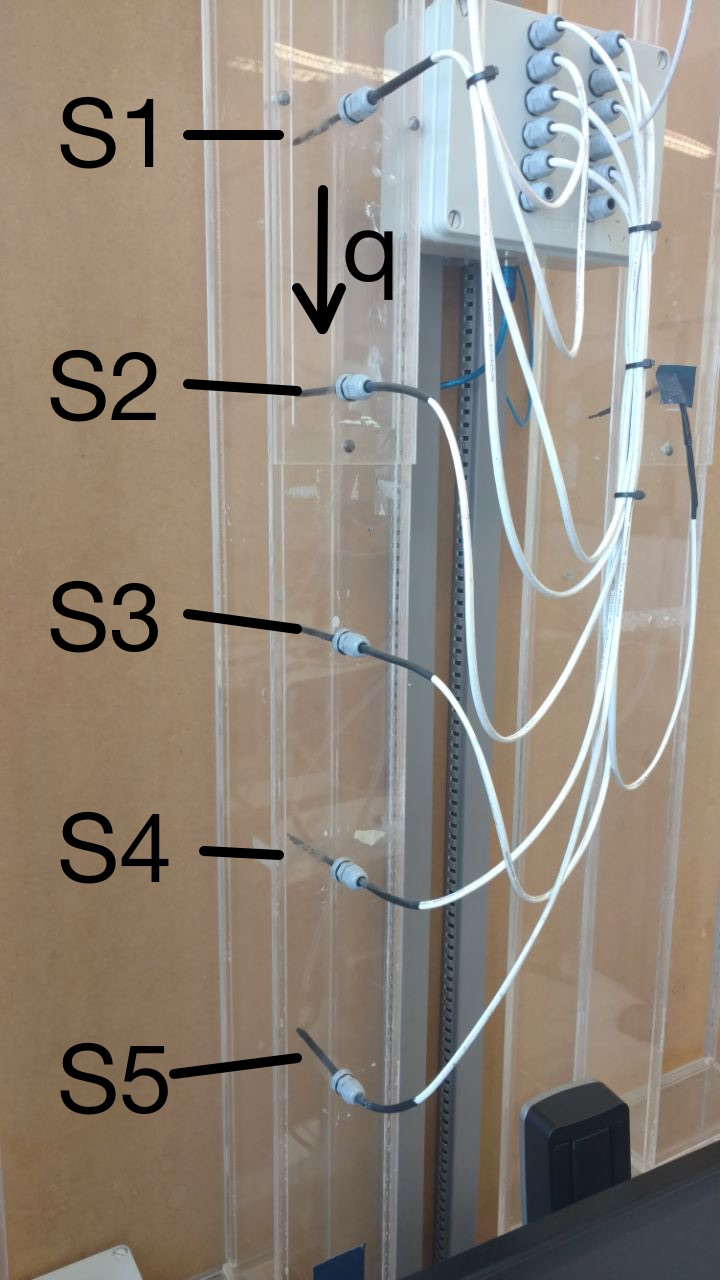
\includegraphics[height=0.5\linewidth]{imgs/planta-spd}
    \caption{Sensores da planta}%
    \label{fig:sensors-spd}
\end{figure}

O observador é um sistema que estima os estados de um modelo baseado nas
entradas e saídas do mesmo. O observador de Kalman, também conhecido como filtro
de Kalman, é uma formulação que permite estimar o modelo de forma precisa mesmo
na presenta de ruídos, seja na leitura da saída ou dos próprios estados.

O uso de controladores MPC com modelos SPD não é novo. Sua maior aplicação, no
entanto, continua sendo na área da química e fabricação de aço. Assim esta
proposta visa o desenvolvimento de um controlador que utiliza técnicas
conhecidas de uma maneira não convencional. Espera-se com isto mostrar a
eficiência desta combinação (\textcite{article:shang}).

Em ambientes industriais é comum o uso de computadores lógicos programáveis para
fazer a interface com o hardware. No meio acadêmico, no entanto, utiliza-se
softwares como o \textit{MATLAB} e \textit{LabVIEW} para a prototipagem rápida.
Isto requer que o pesquisador recrie a interface gráfica e controle a aquisição
de dados manualmente, o que consome tempo que poderia ser gasto com a pesquisa.

Assim, uma plataforma que faça a interface com o hardware e possibilite a
execução de um controlador de forma transparente permite que o pesquisador se
concentre nestes estudos e não se preocupe com detalhes da implementação da
aquisição dos dados. Tal ferramenta também permitiria ao pesquisador
interagir com CLPs, desenvolvendo e testando controladores de forma fácil em
uma linguagem simples (Python) sem se preocupar com todas as nuâncias das
linguagens LADDER utilizadas nos PLCs, podendo implementar seu controlador nesta
linguagem limitada apenas ao final, quando este tiver sido devidamente testado.

A aplicação de uma plataforma para controle em todos as plantas do laboratório
permite que os usuários possam migrar de uma planta para outra sem dificuldades.
Também permite que controladores e observadores desenvolvidos sejam testados em
diferentes plantas com poucas modificações, já que as interfaces seriam as
mesmas em todas elas.

\noindent
{\textbf Áreas envolvidas}

A principal área deste trabalho é controle, por ter o maior peso teórico e de
desenvolvimento. No entanto o trabalho também contempla as áreas de elétrica,
pelas modificações que serão feitas na eletrônica de acionamento e aquisição de
dados do forno, e computação, pelas modificações que serão feitas na plataforma
de controle para que esta possa se comunicar com o hardware e as modificações
que serão feitas para corrigir defeitos e implementar melhorias, como, por
exemplo, recuperar o erro do banco de dados e exibir para o usuário e, caso
possível, gerar mensagens de erro mais informativas, que apontam o lugar do
erro.

  \cleardoublepage{}
  % !TeX root = document.tex
% !TeX encoding = UTF-8 Unicode

\chapter{Objetivos}%
\label{chp:objectives}

Desenvolver um controlador do tipo MPC com restrições com modelo SPD utilizando
observadores do tipo Kalman e implementá-lo utilizando e adaptando a plataforma
de controle desenvolvida pelo proponente para uso no forno do laboratório de
sinais e sistemas. O objetivo pode ser assim dividido:

\begin{itemize}
      \item modificar a eletrônica da planta: instalar circuitos
            microprocessados com o intuito de controlar o acionamento do forno,
            fornecendo um caminho alternativo ao acionamento que já está
            implementado e permitindo a integração com a plataforma de controle;
      \item modificar a plataforma de controle: desenvolver driver específico
            para o forno, de forma a tornar o acionamento dos atuadores e a
            leitura dos sensores mais simples e direto para os futuros usuários;
      \item desenvolver o controlador MPC\@: utilizar o modelo SPD desenvolvido
            pelo~\textcite{masterthesis:nelson} para desenvolver um
            controlador MPC com restrições na entrada e saída de forma a
            controlar a temperatura em um ponto diferente daquele onde está
            fisicamente instalado o sensor;
      \item implementar o controlador: utilizar a linguagem Python e a
            plataforma de controle para implementar o controlador e executar o
            controle da planta;
      \item comparar o desempenho do controlador: usar índices de desempenho
            para comparar o desempenho do controlador MPC com controladores PI a
            serem desenvolvidos utilizando as técnicas
            de~\textcite{article:clarke} e~\textcite{article:martins};
      \item realizar melhorias na plataforma: ao utilizar a plataforma como
            usuário, espera-se encontrar dificuldades, erros e novas ideias que
            serão ser corrigidos/implementadas, como, por exemplo, recuperação
            de mensagens de erro salvas no banco de dados e exibição para o
            usuário e verificação de sintaxe de código digitado pelo usuário.
\end{itemize}

  \cleardoublepage{}
  % !TeX root = document.tex
% !TeX encoding = UTF-8 Unicode

\chapter{Metodologia}%
\label{chp:methodology}

Para que a plataforma de controle possa se comunicar com o forno do laboratório
de sinais e sistemas foi necessário modificar o circuito de acionamento da
mesma. Para isso foram utilizados circuitos microcontrolados que se comunicam
com o circuito de acionamento e sensoriamento presente na mesma.

Esse novo circuito foi programado para se comunicar com a plataforma de
controle. Um \textit{driver} foi escrito para a mesma para permitir o controle
dos atuadores e leitura dos sensores de forma transparente e específica para
este sistema. O \textit{driver} abstrai a interface com o hardware de forma que
o usuário não precise se preocupar com detalhes da implementação, como número de
porta e pino, tensões de operação, etc.

Também foi necessário calibrar todos os sensores e atuadores, além de confererir
o funcionamento dos circuitos elétricos. Todo este procedimento foi feito
usando-se a plataforma de controle para a aquisição de dados. Para isso foi
necessário estudar os trabalhos de~\textcite{misc:nelson}
e~\textcite{misc:valle-silva}.

Os modelos levantados por~\textcite{masterthesis:nelson} foram validados no
sistema físico. Isto foi necessário para verificar que não houve alterações
significativas no sistema desde o seu desenvolvimento. Para o uso destes modelos
foi necessário estudar sobre sistemas a parâmetros distribuídos e observadores
de Kalman.

O controlador MPC utilizado é discreto no tempo e baseado em modelo em espaço de
estados, logo foi necessário estudar sobre controle digital e modelagem em
espaço de estados, além da própria técnica de controle. Para isto foram
utilizados, principalmente, os livros do~\textcite{book:dorf},
do~\textcite{book:ogata}, do~\textcite{book:wang} e as notas de aula do
Professor~\textcite{misc:patwardhan}.

Para o desenvolvimento do controlador foi utilizado o modelo SPD além de
determinadas restrições do sinal de controle. Os estados utilizados no
controlador são os provenientes do observador do tipo Kalman utilizado
pelo~\textcite{masterthesis:nelson}.

Para comparar o desempenho do controlador MPC foram desenvolvidos controladores
PI por síntese direta. Utilizou-se os índices \(IAE\) e \(IA\Delta{}X\) para
realizar uma comparação quantitativa dos controladores.

Todos os controladores foram implementados utilizando a plataforma de controle e
a linguagem de programação Python, assim como todos os testes que que usem o
acionamento do forno e/ou medição de seus termômetros. Desta forma foram
corrigidos na plataforma todos os problemas percebidos na mesma do ponto de
vista de usuário. Também foram implementadas várias novas funcionalidades,
visando seu aperfeiçoamento.

  \cleardoublepage{}
  % !TeX root = document.tex
% !TeX encoding = UTF-8 Unicode

\chapter{Fundamentação Teórica}%
\label{chp:foundations}

Para a realização deste trabalho é necessário conhecimento nas áreas de controle
preditivo por modelo e sistemas a parâmetros distribuídos. Este capítulo visa
explicar sucintamente esses conceitos.

\section{Controlador preditivo por modelo}%
\label{sec:mpc}

Controle preditivo por modelo é uma técnica comumente utlizada pelas indústrias
petroquímica, farmacêutica e do aço. Ela utiliza o modelo para prever a saída do
sistema e, com isso, otimizar a trajetória do sinal de
controle~\cite{book:wang}.

\subsection{Princípio de funcionamento}%
\label{subsec:mpc-basic}

A formualção \ac{MPC} mais comum é a em espaço de estados. Um modelo em espaço
de estados tem a forma

\begin{equation}
	\label{eq:ss}
	\begin{split}
		\dot{x}(t) = A x(t) + B u(t), \\
		y(t) = C x(t) + Du(t),
	\end{split}
\end{equation}

onde \( A \in R^{n \times n} \) é a matriz dinâmica do sistema, \( B in R^{n
\times m} \) e a matriz de entrada, \( C \in R^{m \times n} \) é a matriz de
saída. \( D \in R^{m \times m} \) é normalente \( 0 \). \( x(t) \in R^{m \times
1} \) é o vetor de estados e \( u(t) \in R^{m \times 1} \) são as entradas do
sistema no instante \( t \).

Neste trabalho será utilizada a formulação discreta do controlador preditivo.
Esta formulação tem a vantagem de poder ser implementada facilmente em
dispositivos digitais, além de permitir certo controle do tempo de amostragem.

Ao discretizar um sistema altera-se sua formulação para que a matriz de dinâmica
do sistema não mais produza a variação do estado, mas sim o valor do estado após
\( \Delta{}t \) segundos. Um intervalo de tempo de \( \Delta{}t \) segundos é
chamado de instante, sendo \( t = k\Delta{}t \). Para discretizar um modelo em
espaço de estados usa-se a equação~\eqref{eq:discretize-ss}.

\begin{equation}
	\label{eq:discretize-ss}
	x(k+1) = e^{AT} x(k) + \int^T_0{e^{At}dt}B u(k)
\end{equation}

Ao discretizar o modelo~\eqref{eq:ss} utilizando~\eqref{eq:discretize-ss}
obtem-se~\eqref{eq:discrete-ss}.

\begin{equation}
	\label{eq:discrete-ss}
	\begin{split}
		x(k+1) = A x(k) + B u(k), \\
		y(k) = C x(k) + Du(k).
	\end{split}
\end{equation}

Uma vez obtido o modelo discreto o mesmo deve ser aumentado com um integrador.
Para inserir um integrador no sistema utiliza-se a
equação~\eqref{eq:augment-matrix}.

\begin{equation}
	\label{eq:augment-matrix}
	\begin{bmatrix}
		\Delta x(k+1) \\
		y(k+1)
	\end{bmatrix} =
	\begin{bmatrix}
		A         & 0_m^T \\
		C\cdot{}A & 1
	\end{bmatrix}
	\begin{bmatrix}
		\Delta x(k) \\
		y(k)
	\end{bmatrix} +
	\begin{bmatrix}
		B \\
		C\cdot{}B
	\end{bmatrix}
	\Delta u(k)
\end{equation}

Observe que os estados e o sinal de entrada foram substituídos pro variações dos
mesmos. Isso é possível pois

\begin{equation}
	\Delta x(k+1) = A \Delta x(k) + B \Delta u(k),
\end{equation}

e é também necessário para o funcionamento do controlador. O motivo para esta
reformulação será percebido mais adiante.

Uma vantagem do modelo em espaço de estados discreto é que é possível calcular
estados futuros facilmente, sem a necessidade de se resolver uma equação
diferencial. Utilizando deste fato pode-se utilizar o
modelo~\eqref{eq:discrete-ss} para obter uma equação da próxima saída do
sistema, através da substituição de \( x(k) \) por \( x(k+1) \) na equação da
saída:

\begin{equation}
	\label{eq:first-output}
	y(k+1) = C ( A x(k) + B u(k) ).
\end{equation}

Ao realizar esta substituição uma segunda vez, obtém-se a saída do sistema após
2 instantes:

\begin{equation}
	\label{eq:second-output}
	y(k+2) = C ( A ( A x(k) + B u(k) ) + B u(k+1) ).
\end{equation}

Com uma nova subsituição obtém-se a saída após 3 instantes:

\begin{equation}
	\label{eq:third-output}
	y(k+3) = C ( A ( A ( A x(k) + B u(k) ) + B u(k+1) ) + B u(k+2) ).
\end{equation}

Tem-se então que a saída depende do estado atual e da trajetória de controle.
Reescrendo estas equações de forma matricial para qualquer número \( N_p \) de
saídas futuras e \( N_c\) de entradas futuras, tem-se

\begin{equation}
	\label{eq:Y}
	Y = F x(k) + \Phi U
\end{equation}

onde

\begin{equation}
	\begin{split}
		Y=
		\begin{bmatrix}
			y(k+1)   \\
			y(k+2)   \\
			y(k+3)   \\
			\vdots{} \\
			y(k+N_p) \\
		\end{bmatrix};
		F=
		\begin{bmatrix}
			CA       \\
			CA^2     \\
			CA^3     \\
			\vdots{} \\
			CA^{N_p} \\
		\end{bmatrix};
		U=
		\begin{bmatrix}
			u(k+1)   \\
			u(k+2)   \\
			u(k+3)   \\
			\vdots{} \\
			u(k+N_c) \\
		\end{bmatrix};
		\\
		\\
		\Phi=
		\begin{bmatrix}
			CB          & 0           & 0           & \hdots{} & 0             \\
			CAB         & CB          & 0           & \hdots{} & 0             \\
			CA^2B       & CAB         & CB          & \hdots{} & 0             \\
			\vdots{}    &             &             &          &               \\
			CA^{N_p-1}B & CA^{N_p-2}B & CA^{N_p-3}B & \hdots{} & CA^{N_p-N_c}B \\
		\end{bmatrix}
	\end{split}
\end{equation}

No entanto, para que essa formulação funcione devemos ter \( N_c = N_p \). Isto
no entanto não é desejado. Por questões de implementação computacional e
matemáticas é preferível que \( N_c \ll N_p \). Isso se torna possível se
substituirmos \( U \) por \( \Delta{}U \), o que é feito na matriz aumentada.
Essa substituição é possível, pois, devido à presença do integrador, um valor de
\( \Delta{}U = 0 \) significa que o último sinal aplicado é mantido.

Para compreender melhor este conceito tome com exemplo um sistema de tanques
onde deseja-se controlar o nível alterando-se a vazão de uma bomba. Para todo
\( N_p > N_c \) tem-se uma vazão de 0, ou seja, a bomba seria desligada. Isso
faria com que o nível caísse toda vez que o sistema alcançasse o equilíbrio.
Utilizando \( \Delta{}U \) o valor zero significa manter a última vazão apicada,
o que faz com que o sistema permaneça em equilíbrio uma vez que o sinal de
controle seja zerado.

MPC é uma técnica baseada em otimização. Problemas de otimização são resolvidos
encontrando-se o máximo ou mínimo de alguma função. Deve-se então definir uma
função que, ao ser minimizada, terá como resultado a trajetória ótima. Este tipo
de função é chamada de função de custo e normalmente utiliza-se em \ac{MPC} uma
função quadrática, o que garante a convergência. Escrevendo a função com o
intuito de minimizar o erro em regime permanente e a variação do sinal de
controle, tem-se

\begin{equation}
	\label{eq:cost-function}
	J = {(R_s - Y)}^T(R_s-Y) + \Delta{}U^T\bar{R}\Delta{}U,
\end{equation}

onde \( R_s \) é o vetor referência com a mesma dimensão do vetor \( Y \) e
\(\bar{R} \) é uma variável que pode ser usada para controlar o peso da variação
do sinal de controle. \( \bar{R} \) maior implica em variações menores.
Substituindo~\eqref{eq:Y} em~\eqref{eq:cost-function} tem-se

\begin{equation}
	J = {(R_s-Fx(k))}^T(R_s-Fx(k))-2\Delta{}U^T\Phi^T(R_s-Fx(k))+\Delta{}U^T(\Phi^T\Phi+\bar{R})\Delta{}U.
\end{equation}

Derivando em função da variação do sinal de controle, \( \Delta{}U \):

\begin{equation}
	\frac{\partial{}J}{\partial{}\Delta{}U} = -2\Phi^T(R_s-Fx(k))+2(\Phi^T\Phi+\bar{R})\Delta{}U.
\end{equation}

Igualando \( \frac{\partial{}J}{\partial{}\Delta{}U} \) a zero e isolando \(
\Delta{}U \):

\begin{equation}
	\label{eq:delta-u}
	\Delta{}U = {(\Phi^T\Phi+\bar{R})}^{-1}\Phi^T(R_s-Fx(k)).
\end{equation}

Ao utilizar \( N_c = N_p \), é possível, através da equação~\eqref{eq:delta-u},
encontrar os valores ótimos de \( \Delta{}U \) que farão o sistema seguir uma
referência. No entanto, o controlador não será capaz de rejeitar ruídos.
Aplicando apenas o primeiro sinal de controle, medindo ou estimando os estados
do sistema e recalculando a trajetória a cada instante é possível contornar este
problema.

Esta é a formulação básica do MPC, porém ela não fornece o que pode ser
considerada a maior vantagem desta técnica de controle: restrição do sinal de
controle, da saída, de estados ou de suas variações. Para isto é necessário
voltar na função de custo e resolvê-la de uma maneira que permita a inserção
de restrições no equacionamento.

\pagebreak

\subsection{Restrições de parâmetros}%
\label{subsec:mpc-restricted}

Os parâmetros mais comumente restringidos são a saída do sistema, o sinal de
controle e a variação do sinal de controle. Estas restrições tem a forma de
inequações e podem ser escritas como

\begin{equation}
	\label{eq:generic-restriction-u}
	U^{\min} \le U \le U^{\max},
\end{equation}

\begin{equation}
	\label{eq:generic-restriction-y}
	Y^{\min} \le Y \le Y^{\max},
\end{equation}

e

\begin{equation}
	\label{eq:generic-restriction-du}
	\Delta{}U^{\min} \le \Delta{}U \le \Delta{}U^{\max}.
\end{equation}

Usando a equação~\eqref{eq:generic-restriction-du} como exemplo, pode-se
reescrevê-la como duas inequações:

\begin{equation}
	\label{eq:generic-restriction-du-two-eq}
	\begin{split}
		-\Delta{}U \le -\Delta{}U^{\min} \\
		\Delta{}U \le \Delta{}U^{\max}.
	\end{split}
\end{equation}

Em forma matricial,

\begin{equation}
	\label{eq:generic-restriction-du-matrix-form}
	\begin{bmatrix}
		-I \\
		I
	\end{bmatrix} \Delta{}U \le
	\begin{bmatrix}
		-\Delta{}U^{\min} \\
		\Delta{}U^{\max}
	\end{bmatrix}.
\end{equation}

Para os casos de Y e U, deve-se fazer as devidas substituições de forma que a
variável \( \Delta{}U \) apareça na inequação. Esta substituição é necessária
pois a técnica de otimização irá buscar a solução ótima para apenas uma variável
(\( \Delta{}U \)), sendo necessário que todas as restrições sejam funções desta
variável.

Para \( Y \) deve-se substituir a equação~\eqref{eq:Y}
em~\eqref{eq:generic-restriction-y}, isolar \( \Phi{}\Delta{}U \) e reescrevê-la
de forma matricial:

\begin{equation}
	\label{eq:generic-restriction-y-matrix-form}
	\begin{bmatrix}
		-\Phi \\
		\Phi
	\end{bmatrix} \Delta{}U \le
	\begin{bmatrix}
		-Y^{\min} + Fx(k) \\
		Y^{\max} - Fx(k)
	\end{bmatrix}.
\end{equation}

Para a restrição de \( U \), lembrando que \( u(k) = u(k-1) + \Delta{}u(k) \),
tem-se

\begin{equation}
	\label{eq:generic-restriction-u-matrix-eq}
	\begin{bmatrix}
		u(k)   \\
		u(k+1) \\
		\vdots \\
		u(k+N_c-1)
	\end{bmatrix} =
	\begin{bmatrix}
		I      \\
		I      \\
		\vdots \\
		I
	\end{bmatrix}
	u(k-1) +
	\begin{bmatrix}
		I & 0 & \hdots & 0 \\
		I & I & \hdots & 0 \\
		\vdots             \\
		I & I & \hdots & I \\
	\end{bmatrix}
	\begin{bmatrix}
		\Delta{}u(k)       \\
		\Delta{}u(k+1)     \\
		\vdots
		\Delta{}u(k+N_c-1) \\
	\end{bmatrix},
\end{equation}

que pode ser reescrita como

\begin{equation}
	\label{eq:generic-restriction-u-matrix-form}
	\begin{bmatrix}
		-C_1u(k-1) - C_2\Delta{}U \\
		C_1u(k-1) + C_2\Delta{}U  \\
	\end{bmatrix} \le
	\begin{bmatrix}
		-U^{\min} \\
		U^{\max}
	\end{bmatrix}.
\end{equation}

Reduzindo estas restrições em uma única inequação matricial, obtem-se

\begin{equation}
	\label{eq:generic-restriction-matrix}
	\begin{bmatrix}
		M_1 \\
		M_2 \\
		M_3
	\end{bmatrix} \Delta{}U \le
	\begin{bmatrix}
		N_1 \\
		N_2 \\
		N_3
	\end{bmatrix},
\end{equation}

sendo

\begin{equation*}
	\begin{split}
		M_1 =
		\begin{bmatrix}
			-C_2 \\
			C_2
		\end{bmatrix};
		N_1 =
		\begin{bmatrix}
			-U^{\min} + C_1u(k-1) \\
			U^{\max} + C_1u(k-1)  \\
		\end{bmatrix};
		M_2 =
		\begin{bmatrix}
			-I \\
			I
		\end{bmatrix}; \\
		N_2 =
		\begin{bmatrix}
			-\Delta{}U^{\min} \\
			\Delta{}U^{\max}
		\end{bmatrix};
		M_3 =
		\begin{bmatrix}
			-\Phi \\
			\Phi
		\end{bmatrix};
		N_3 =
		\begin{bmatrix}
			-Y^{\min} + Fx(k) \\
			Y^{\max} - Fx(k)
		\end{bmatrix}.
	\end{split}
\end{equation*}

Pode-se inserir outras restrições, como em estados, por exemplo, seguindo essa
lógica de formulação. Obtem-se então todas as restrições descritas na forma

\begin{equation}
	\label{eq:generic-restriction-formulation}
	M\Delta{}U \le \gamma.
\end{equation}

Este formato de restrições é comumente utilizado em problemas de otimização. Os
métodos de programação quadrática, multiplicadores de lagrange e até mesmo o
método SIMPLEX usam restrições escritas nesse formato. Deve-se então escolher um
método de otimização e ajustar a função de custo à aquela necessária para usar o
método. Como a função de custo é quadrática, convém escolher um método que seja
capaz de otimizar problemas quadráticos.

O método de programação quadrática tem uma função de custo que se assemelha à
que foi definida, como pode ser visto na equação~\eqref{eq:cost-function-qp}.
Vale notar que as variáveis e constantes desta função não tem relação com as
variáveis definidas anteriormente, mas são as comumente utilizadas por
matemáticos ao trabalhar com estes métodos.

\begin{equation}
	\label{eq:cost-function-qp}
	J = \frac{1}{2} x^T Ex + x^T F.
\end{equation}

Reescrevendo~\eqref{eq:cost-function} no formato de~\eqref{eq:cost-function-qp},
encontra-se

\begin{equation}
	\label{eq:cost-function-qp-constants}
	\begin{split}
		E = \Phi^T \Phi + \bar{R} \\
		F = \Phi^T (Fx - R_s),
	\end{split}
\end{equation}

no qual \( E \) e \( F \) à esquerda da igualdade vem da
equação~\eqref{eq:cost-function-qp} e \( \Phi \), \( F \), \( R_s \) e \(\bar{R}
\) à direita da igualdade da formulação do \ac{MPC}.

Explicar o funcionamento do método de programação quadrática foge do escopo
deste trabalho. Existem bibliotecas que implementam este método em MATLAB e
Python como, por exemplo, a CVXOPT\footnote{https://cvxopt.org/}. Para usar o
\textit{solver} de programação quadrática definido nessas bibliotecas deve-se
definir as matrizes \( E \), \( F \), \( M \) e \( \gamma \).

Analisando a equação~\eqref{eq:generic-restriction-matrix} pode-se ver que suas
dimensões não são iguais, isto é, a matriz \( M \) não é quadrada. Isso ocorre
pois é possível ter mais restrições do que variáveis. Isso não é um problema já
que as restrições são inequações, logo uma mais de uma restrição pode ser
satisfeita se tentar satisfazer apenas uma delas, mais restritiva.

Em outras palavra, apenas um subconjunto de restrições estará ativo em um dado
momento. Existem técnicas para determinar qual é o conjunto ativo. Isto, no
entanto, não é necessário, já que o \textit{solver} irá encontrar a mesma
solução para o conjunto completo que para o subconjunto ativo de restrições. A
vantagem de encontrar o conjunto ativo é reduzir o custo computacional da
otimização.

\pagebreak

\section{Sistemas a parâmetros distribuídos}%
\label{sec:spd}

Neste trabalho é estudada apenas a abordagem proposta
por~\textcite{masterthesis:nelson}. Ela consiste basicamente em unir duas
propostas já existentes, a SPD por subsistemas interconectados e a baseada em
modelos lineares a parâmetros variantes no espaço (Spatial \ac{LPV}, do inglês
\textit{Spatial Linear Parameter Varying}).

SPD por subsistemas interconectados consiste em modelar um problema que varia no
espaço, ou seja, um \ac{SPD}, utilizando vários sistemas a parâmetros
concentrados. Assim cada \ac{SPC} representa a saída do sistema em um ponto no
espaço. Esta abordagem, no entanto, é limitada, já que os pontos no espaço onde
pode-se fazer a estimação dos estados é fixada pelo modelo. Para fazer a
estimação em outros pontos é necessário remodelar o sistema.

Na Figura~\ref{fig:interconected-subsystems} pode-se ver um esquemático do
funcionamento desta aproximação. O sistema varia no espaço de \( 0 \) a \( L \).
Para obter estados intermediários, desenvolve-se vários modelos que descrevem a
dinâmica de um ponto intermediário \( s_i \) até um ponto \( s_j \), utilizando
modelos \ac{SPC} para tal.

\begin{figure}[ht!]
	\centering
	\captionsetup{justification=centering}
	\begin{tikzpicture}
		% thick line on middle
		\draw[line width=2pt] (0,2) -- (8,2);
            \node[circle,fill,inner sep=2pt,label=above:{$y(s_0,t)$}] at (0,2) {};
            \node[circle,fill,inner sep=2pt,label=above:{$y(s_1,t)$}] at (2,2) {};
            \node[circle,fill,inner sep=2pt,label=above:{$y(s_2,t)$}] at (4,2) {};
            \node at (6,2.3) {$\hdots$};
            \node[circle,fill,inner sep=2pt,label=above:{$y(s_n,t)$}] at (8,2) {};
		% s indicator on top
		\draw(0,3) -- (0,3.5);
		\draw[->] (0,3.25) -- (1,3.25);
		\node at (0.5,3.5) {$s$};
		% line on bottom
		\draw(0,0) -- (8,0);
		\draw(0,0.25) -- (0,-0.25);
		\draw(8,0.25) -- (8,-0.25);
		\node at (0,-0.5) {$0$};
		\node at (8,-0.5) {$L$};
		% arrow in middle
		\node at (4,1.7) {$s$};
		\draw[<->] (3.5,1.5) -- (4.5,1.5);
		% u line
		\draw[->] (0,1) -- (0,1.9);
            \node at (0.7,1.5) {$u(0,t)$};
            % blocks
            \node[draw,text width=5pt,text height=5pt] at (0.0,-2) (s0) {};
            \node[draw,text width=5pt,text height=5pt] at (2,-2) (s1) {};
            \node[draw,text width=5pt,text height=5pt] at (3.8,-2) (s2) {};
            \node at (5.75,-2) (s3) {$\hdots$};
            \node[draw,text width=5pt,text height=5pt] at (8.0,-2) (s4) {};
            \draw[->] (-1.5,-2) -- node[above] {$u(0,t)$} ++ (s0);
            \draw[->] (s0) -- node[above] {$y(s_0,t)$} ++ (s1);
            \draw[->] (s1) -- node[above] {$y(s_1,t)$} ++ (s2);
            \draw[->] (s2) -- node[above] {$y(s_2,t)$} ++ (s3);
            \draw[->] (s3) -- node[above] {$y(s_{n-1},t)$} ++ (s4);
	\end{tikzpicture}
	\caption{Subsistemas interconectados}%
	\label{fig:interconected-subsystems}
\end{figure}

Já o método de modelos lineares a parâmetros variantes no espaço propõe a
criação de um modelo que irá descrever a dinâmica do sistema do ponto inicial
até determinado ponto espacial que é definido como uma variável, chamada de
\textit{scheduling}. Assim, alterando esta variável obtém-se como saída o estado
em um ponto diferente no espaço.

A figura~\ref{fig:lpv-system} contém o esquemático de um modelo \ac{LPV}. Nele o
mesmo sistema é descrito por apenas um modelo que tem um parâmetro que altera o
ponto no espaço ao qual a saída se refere. Assim pode-se obter o estado em
vários pontos no espaço sem a necessidade de remodelar o sistema.

\begin{figure}[ht!]
	\centering
	\captionsetup{justification=centering}
	\begin{tikzpicture}
		% thick line on middle
		\draw[line width=2pt] (0,2) -- (8,2);
            \node[circle,fill,inner sep=2pt,label=above:{$y(s_0,t)$}] at (0,2) {};
            \node[circle,fill,inner sep=2pt,label=above:{$y(s_1,t)$}] at (2,2) {};
            \node[circle,fill,inner sep=2pt,label=above:{$y(s_2,t)$}] at (4,2) {};
            \node at (6,2.3) {$\hdots$};
            \node[circle,fill,inner sep=2pt,label=above:{$y(s_n,t)$}] at (8,2) {};
		% s indicator on top
		\draw(0,3) -- (0,3.5);
		\draw[->] (0,3.25) -- (1,3.25);
		\node at (0.5,3.5) {$s$};
		% line on bottom
		\draw(0,0) -- (8,0);
		\draw(0,0.25) -- (0,-0.25);
		\draw(8,0.25) -- (8,-0.25);
		\node at (0,-0.5) {$0$};
		\node at (8,-0.5) {$L$};
		% arrow in middle
		\node at (4,1.7) {$s$};
		\draw[<->] (3.5,1.5) -- (4.5,1.5);
		% u line
		\draw[->] (0,1) -- (0,1.9);
            \node at (0.7,1.5) {$u(0,t)$};
            % blocks
            %% s0
            \node[draw,text width=5pt,text height=5pt] at (0,-2) (s0) {};
            \node[text width=5pt,text height=5pt] at (2,-2) (s0e) {};
            \draw[->] (-1.5,-2) -- node[above] {$u(0,t)$} ++ (s0);
            \draw[->] (s0) -- node[above] {$y(s_0,t)$} ++ (s0e);
            %% s1
            \node[draw,text width=2cm,text height=5pt] at (1,-4) (s1) {};
            \node[text width=5pt,text height=5pt] at (4,-4) (s1e) {};
            \draw[->] (-1.5,-4) -- node[above] {$u(0,t)$} ++ (s1);
            \draw[->] (s1) -- node[above] {$y(s_1,t)$} ++ (s1e);
            %% s2
            \node[draw,text width=4cm,text height=5pt] at (2,-6) (s2) {};
            \node[text width=5pt,text height=5pt] at (6,-6) (s2e) {};
            \draw[->] (-1.5,-6) -- node[above] {$u(0,t)$} ++ (s2);
            \draw[->] (s2) -- node[above] {$y(s_2,t)$} ++ (s2e);
            %% sn
            \node[draw,text width=8cm,text height=5pt] at (4,-8) (sn) {};
            \node[text width=5pt,text height=5pt] at (10,-8) (sne) {};
            \draw[->] (-1.5,-8) -- node[above] {$u(0,t)$} ++ (sn);
            \draw[->] (sn) -- node[above] {$y(s_n,t)$} ++ (sne);
	\end{tikzpicture}
	\caption{Subsistema LPV}%
	\label{fig:lpv-system}
\end{figure}

Ao combinar as duas técnicas,~\textcite{masterthesis:nelson} propõe que se use
dois modelos \ac{LPV} complementares como subsistemas interconectados. O
primeiro modelo descreve a dinâmica do sistema do atuador até um ponto \( x \)
enquanto o segundo modelo descreve a dinâmica desse ponto até uma saída fixa.

Um esquemático desta técnica é apresentado na figura~\ref{fig:nelson-system}.
Nele pode-se ver que foi utilizado a técnica de subsistemas interconectados, no
entanto, os subsistemas utilizados são \ac{LPV} e complementares. Isso significa
que ao alterar o valor da variável \( s_l \) altera-se ambos sistemas para que o
primeiro forneça o estado em \( s_l \) e o segundo a saída em \( L \), dada a
saída \( s_l \). Desta forma o ponto \( s_l \) é móvel, podendo ser alterado a
qualquer momento.

\begin{figure}[ht!]
	\centering
	\captionsetup{justification=centering}
	\begin{tikzpicture}
		% thick line on middle
		\draw[line width=2pt] (0,2) -- (8,2);
            \node[circle,fill,inner sep=2pt,label=above:{$y(0,t)$}] at (0,2) {};
            \node[circle,fill,inner sep=2pt,label=above:{$y(s_l,t)$}] at (4,2) {};
            \node[circle,fill,inner sep=2pt,label=above:{$y(L,t)$}] at (8,2) {};
		% s indicator on top
		\draw(0,3) -- (0,3.5);
		\draw[->] (0,3.25) -- (1,3.25);
		\node at (0.5,3.5) {$s$};
		% line on bottom
		\draw(0,0) -- (8,0);
		\draw(0,0.25) -- (0,-0.25);
		\draw(8,0.25) -- (8,-0.25);
		\node at (0,-0.5) {$0$};
		\node at (8,-0.5) {$L$};
		% arrow in middle
		\node at (4,1.7) {$s$};
		\draw[<->] (3.5,1.5) -- (4.5,1.5);
		% u line
		\draw[->] (0,1) -- (0,1.9);
            \node at (0.7,1.5) {$u(0,t)$};
            % blocks
            \node[draw,text width=3cm,text height=5pt] at (1.5,-2) (sl) {};
            \node[draw,text width=3cm,text height=5pt] at (6.5,-2) (sl2) {};
            \draw[->] (-1.5,-2) -- node[above] {$u(0,t)$} ++ (sl);
            \draw[->] (sl) -- node[above] {$y(s_l,t)$} ++ (sl2);
            \node[text width=5pt,text height=5pt] at (10,-2) (sl2e) {};
            \draw[->] (sl2) -- node[above] {$y(L,t)$} ++ (sl2e);
	\end{tikzpicture}
	\caption{Subsistemas LPV interconectados}%
	\label{fig:nelson-system}
\end{figure}

A principal vantagem desta abordagem é poder utilizar um sensor na saída do
segundo modelo LPV e utilizar um observador para estimar o estado de qualquer
ponto entre o atuador e o sensor, selecionando o ponto através apenas da
alteração da variável \textit{scheduling}, \( s_l \).

\subsection{Modelagem do forno por LPVs interconectados}%
\label{subsec:lpv-oven}

Para modelar o sistema foram utilizados dois modelos \ac{ARMAX} (Modelo
autoregressivo de média variável com entradas exógenas, do inglês
\textit{Autoregressive–moving-average with exogenous inputs}), um de \( 0 \) até
\( s_\ell \) e outro de \( s_\ell \) até \( L \). A formulação geral para estes
modelos é

\begin{equation}
	\label{eq:lpv-polynom-generic-sl}
	\begin{split}
		y(s_\ell,k) = -\sum_{i_y=1}^{n_y}a_{i_y}(s_\ell)y(0,k-i_y)
					+\sum_{i_u=n_k}^{n_k+n_u-1}b_{i_u}(s_\ell)y(s_\ell,k-i_u) \\
					+\sum_{i_v=1}^{n_v}c_{i_v}(s_\ell)v(s_\ell,k-i_v)+v(s_\ell,k)
	\end{split}
\end{equation}

e

\begin{equation}
	\label{eq:lpv-polynom-generic-L}
	\begin{split}
		y(L,k) = -\sum_{i_y=1}^{n_y}\alpha{}_{i_y}(\bar{s_\ell})y(L,k-i_y)
					+\sum_{i_u=n_k}^{n_k+n_u-1}\beta{}_{i_u}(\bar{s_\ell})y(\bar{s_\ell},k-i_u) \\
					+\sum_{i_v=1}^{n_v}\gamma{}_{i_v}(\bar{s_\ell})v(\bar{s_\ell},k-i_v)+v(\bar{s_\ell},k).
	\end{split}
\end{equation}

Após um dimencionamento inicial obtém-se

\begin{equation}
	\label{eq:lpv-polynom-sl}
	\begin{split}
		y(s_\ell,k) = -a_1(s_\ell)y(s_\ell,k-1) + b_1(s_\ell)y(0,k-1) \\
					+ c_1(s_\ell)v(s_\ell,k-1) + c_2(s_\ell)v(s_\ell,k-2)
					+ v(s_\ell,k)
	\end{split}
\end{equation}

e

\begin{equation}
	\label{eq:lpv-polynom-L}
	\begin{split}
		y(L,k) = -\alpha{}_1(\bar{s_\ell})y(L,k-1)
					+ \beta{}_0(\bar{s_\ell})y(\bar{s_\ell},k)
					+ \beta{}_1(\bar{s_\ell})y(\bar{s_\ell},k-1) \\
					+ \gamma{}_1(\bar{s_\ell})v(\bar{s_\ell},k-1)
					+ \gamma{}_2(\bar{s_\ell})v(\bar{s_\ell},k-2)
					+ v(\bar{s_\ell},k),
	\end{split}
\end{equation}

sendo os coeficientes na forma

\begin{equation}
	\label{eq:lpv-coeffs-form}
	\begin{split}
		a(s_\ell)=\sum_{i_a=0}^{n_a}a_{i_a}s_{\ell}^{i_a}.
	\end{split}
\end{equation}

Obtém-se assim as funções scheduling de 3~\eqref{eq:lpv-fs3},
5~\eqref{eq:lpv-fs5} e 9~\eqref{eq:lpv-fs9} posições, obtidas utilizando a
técnica de mínimos quadrados para ajustar os coeficientes.

\begin{equation}
	\label{eq:lpv-fs3}
	\begin{split}
		b1 = 1.3291*10^{-9} s_\ell^2 - 2.2196*10^{-5} s_\ell + 0.0563  \\
		a1 = -1.5101*10^{-8} s_\ell^2 + 1.3591*10^{-5} s_\ell - 0.9118 \\
		w1 = 1.6636*10^{-8} s_\ell^2 - 3.2243*10^{-5} s_\ell + 0.0213  \\
		\beta_0 = -2.5839*10^{-4} \bar{s_\ell} + 0.9036                \\
		\beta_1 = 2.3909*10^{-4} \bar{s_\ell} - 0.8628                 \\
		\alpha_1 = -1.6436*10^{-5} \bar{s_\ell} - 0.9559               \\
		w2 = 4.9739*10^{-6} \bar{s_\ell} + 0.0029
	\end{split}
\end{equation}

\begin{equation}
	\label{eq:lpv-fs5}
	\begin{split}
		b1 = -3.3299*10^{-9} * sl^2 - 1.5982*10^{-5} * sl + 0.05711                         \\
		a1 = -3.0164*10^{-8} * sl^2 + 3.3929*10^{-5} * sl - 0.91092                         \\
		w1 = 1.4014*10^{-8} * sl^2 - 2.6372*10^{-5} * sl + 0.01952                          \\
		\beta_0 = -4.8261*10^{-8} * \bar{s_\ell}^2 - 1.3554*10^{-4} * \bar{s_\ell} + 0.8171 \\
		\beta_1 = 5.7969*10^{-8} * \bar{s_\ell}^2 + 8.1357*10^{-5} * \bar{s_\ell} - 0.7485  \\
		\alpha_1 = 2.9771*10^{-8} * \bar{s_\ell}^2 - 8.6561*10^{-5} * \bar{s_\ell} - 0.9149 \\
		w2 = 3.8259*10^{-9} * \bar{s_\ell}^2 - 3.1247*10^{-6} * \bar{s_\ell} + 0.0068
	\end{split}
\end{equation}

\begin{equation}
	\label{eq:lpv-fs9}
	\begin{split}
		b1 = -4.2490*10^{-12} * sl^3 + 3.4291*10^{-9} * sl^2 - 1.5999*10^{-5} * sl + 0.0568                                     \\
		a1 = 9.5100*10^{-12} * sl^3 - 4.7554*10^{-8} * sl^2 + 4.3890*10^{-5} * sl - 0.9112                                      \\
		w1 = -2.3370*10^{-11} * sl^3 + 6.6704*10^{-8} * sl^2 - 5.7759*10^{-5} * sl + 0.0237                                     \\
		\beta_0 = 2.0229*10^{-10} * \bar{s_\ell}^3 - 4.7445*10^{-7} * \bar{s_\ell}^2 + 1.1916*10^{-4} * \bar{s_\ell} + 0.7532   \\
		\beta_1 = -2.5343*10^{-10} * \bar{s_\ell}^3 + 6.2283*10^{-7} * \bar{s_\ell}^2 - 2.8674*10^{-4} * \bar{s_\ell} - 0.6551  \\
		\alpha_1 = -5.5237*10^{-11} * \bar{s_\ell}^3 + 1.4785*10^{-7} * \bar{s_\ell}^2 - 1.5578*10^{-4} * \bar{s_\ell} - 0.8992 \\
		w2 = 8.1120*10^{-11} * \bar{s_\ell}^3 - 1.8802*10^{-8} * \bar{s_\ell}^2 + 1.6462*10^{-4} * \bar{s_\ell} + 0.0017
	\end{split}
\end{equation}

As equações~\eqref{eq:lpv-polynom-L} e~\eqref{eq:lpv-polynom-sl} podem ser
reescritas no formato de espaço de estados como

\begin{equation}
	\label{eq:lpv-ss}
	\begin{split}
		x(k) = 
		\begin{bmatrix}
			x_1(L,k) \\
			x_2(s_\ell,k)
		\end{bmatrix} \\
		x(k+1) =
		\begin{bmatrix}
			-\alpha{}(\bar{s_\ell}) &  \beta_1(\bar{s_\ell}) - \beta_0(\bar{s_\ell})a_1(s_\ell) \\
			0                       & -\alpha{}(s_\ell)
		\end{bmatrix}
		x(k) +
		\begin{bmatrix}
			\beta_0(\bar{s_\ell})b_1(s_\ell) \\
			b_1(s_\ell)
		\end{bmatrix}
		u(0,k) \\
		y(L,k) = 
		\begin{bmatrix}
			1 & 0
		\end{bmatrix}
		x(k).
	\end{split}
\end{equation}

Os modelos levantados por~\textcite{masterthesis:nelson} estão discretizados com
tempo de amostragem de 5 segundos.

\section{Observadores}%
\label{sec:observers}

Observadore são modelos que reconstroem informação em tempo real. Sua função é
recuperar as informações dos estados a partir do modelo do sistema, a entrada, a
saída e o último estado estimado. Eles funcionam como malha fechada, utilizando
o modelo para predizer o próximo estado e um ganho para corrigir o erro da saída
estimada em relação à saída real.

Existem vários tipos de observadores. Neste trabalho serão utilizados dois: o
filtro de Kalman e o observador exponencial com fator de esquecimento. O filtro
de Kalman é talvez o mais utilizado e funciona tanto como observador quanto
filtro de ruídos. Porém sua formulação requer a covariança das variações dos
estados. Já o observador exponencial requer apenas a covariança da saída e
possui uma variável para ajustar a velocidade de convergência facilmente.

\subsection{Filtro de Kalman}%
\label{subsec:kalman}

O filtro de Kalman é um observador estocástico ótimo discreto no tempo
desenvolvido por~\textcite{Kalman1960}. Assumindo que um sistema passa a estar
sujeito a ruídos gaussianos de média nula e não correlacionados \( v \) e \( w
\), podemos descrever seu comportamento como

\begin{equation}
	\label{eq:observer-noisy-model}
	\begin{split}
		x(k+1) = Ax(k) + Bu(k) + v(k) \\
		y(k) = Cx(k) +Du(k) + w(k).
	\end{split}
\end{equation}

Para sistemas descritos desta forma, o Teorema~\ref{theorem:kalman} define o
observador de Kalman.

\begin{theorem}%
	\label{theorem:kalman}
	Para qualquer sequência de entrada regularmente persistente para o par \(
	(A, C) \) o seguinte sistema:

	\begin{equation}
		\label{eq:kalman-definition}
		\begin{split}
			P(\infty)=A(P(\infty)-P(\infty)C^T{(\Gamma+CP(\infty)C^T)}^{-1}CP(\infty))A^T+\Theta \\
			K_{ob}(\infty)=AP(\infty)C^T{(\Gamma+CP(\infty)C^T)}^{-1} \\
			\hat{x}(k+1) = A\hat{x}(k) + Bu(k) + K_{ob}(\infty)(y(k) - C\hat{x}(k))-Du(k)
		\end{split}
	\end{equation}

	provê um observador  ótimo para o sistema~\eqref{eq:observer-noisy-model}.
\end{theorem}

Na equação~\eqref{eq:kalman-definition}, \( \Gamma \) e \( \Theta \) são as
matrizes de covariança da saída e da variação dos estados, respectivamente. O
primeiro pode ser facilmente medido. Basta realizar uma leitura fix com o sensor
por várias amostras e calcular a covariança do vetor de valores resultantes. O
segundo exige que seja possível medir todos os estados, o que nem sempre
acontece. Sendo possível, mede-se todos os estados em um valor fixo por várias
amostras e calcula-se a covariança da diferença dos estados (\( x(k) - x(k-1) \)
para cada estado). Caso não seja possível deve-se procurar formas de estimar a
covariança ou encontrar valores manualmente que produzam resultados
satisfatórios.

\( P(\infty) \) e \( K_{ob}(\infty) \) são os valores \( P \) e \( K_{ob} \) que
estabilizam as equações, ou seja, os valores em que a saída não mais se altera.
Assim o conjunto de equações~\eqref{eq:kalman-definition} é convergente para os
valores de \( P \) e \( K_{ob} \), e esses podem ser obtidos através do cálculo
iterativo de \( P(\infty) \) até sua convergência.

\subsection{Observador exponencial com fator de esquecimento}%
\label{subsec:exponential-observer}

O observador exponecial com fator de esquecimento\cite{Ticlea2009} também é um
observador do tipo Kalman. Isso pode ser visto em sua estrutura. Sua formulação
é dada pelo Teorema~\ref{theorem:exponential-observer}.

\begin{theorem}%
	\label{theorem:exponential-observer}
	Dado os sistema~\eqref{eq:observer-noisy-model}, e assumindo que uma
	sequência de entrada, \( u(k) \),  é regularmente persistente para o par \(
	(A,C) \) e torna A invertível, então, um observador globalmente
	exponencialmente convergente é dado por:

	\begin{equation}
		\label{eq:exponential-observer-definition}
		\begin{split}
			P(\infty)=\delta^{-1}A(P(\infty)-KCP(\infty))A^T \\
			K_{ob}(\infty)=AP(\infty)C^T{(\Gamma+CP(\infty)C^T)}^{-1} \\
			\hat{x}(k+1) = A\hat{x}(k) + Bu(k) + K_{ob}(\infty)(y(k) - C\hat{x}(k))-Du(k).
		\end{split}
	\end{equation}
\end{theorem}

Na equação~\eqref{eq:exponential-observer-definition}, \( \delta{} \) é um
número real que controla a velocidade de convergência do observador. Quanto
menor \( \delta{} \), mais rápido o observador converge.

\subsection{Observabilidade}%
\label{subsec:observability}

Observabilidade é a medida de quão bem os estados internos de um sistema podem
ser estimados a partir de suas saídas. Formalmente um sistema é dito observável
se para qualquer sequência de estados e sinais de controle, o estado atual pode
ser determinado em tempo finito usando apenas as saídas. Se o sistema não é
observável, então existe pelo menos um estado que não pode ser determinado
apenas pela saída.

Para sistemas invariantes no tempo em espaço de estados com \( n \) estados, se
o posto da matriz \( L_o \) da equação~\eqref{eq:observability-matrix} for igual
a \( n \), o sistema é dito observável. A ideia por traz deste teste é que, se a
matriz contém \( n \) linhas linearmente independentes, então os \( n \) estados
podem ser vistos como combinações lineares da saída.

\begin{equation}
	\label{eq:observability-matrix}
	L_o = \begin{bmatrix}
		C       \\
		CA      \\
		CA^2    \\
		CA^{n-1}
	\end{bmatrix}
\end{equation}

  \cleardoublepage{}
  % !TeX root = document.tex
% !TeX encoding = UTF-8 Unicode

\chapter{Recursos Necessários}%
\label{sec:needed-resources}

Para o novo circuito de acionamento, que será inserido paralelo ao existente,
serão necessários circuitos microcontrolados capazes de medir os valores de
tensão existentes no circuito atual e de se comunicar com um computador. Por
isso optou-se por utilizar placas Arduíno, pois são acessíveis e atendem aos
requisitos.

Também optou-se por utilizar um computador portátil de baixo custo como prova de
conceito, pois a plataforma de controle foi pensada de forma a executar bem o
controlador em um computador com recursos limitados. Para isto escolheu-se
utilizar um \textit{Raspberry Pi}. A comunicação entre o \textit{Raspberry} e os
Arduínos se dará por cabo USB (porta serial emulada), enquanto a comunicação do
\textit{Raspberry} com o exterior se dará por cabo de rede.

Com isso, necessitasse dos seguintes componentes:

\begin{itemize}
      \item 1 Raspberry Pi
      \item 2 Arduínos
      \item \textit{jumpers}
      \item Cabos USB
      \item Cabo de rede
\end{itemize}

Todo software utilizado será \textit{open-source}, como: linguagem Python,
plataforma de controle (Lachesis e Moirai), sistema operacional Raspbian, banco
de dados Mongo DB, ambiente de virtualização Docker, suítes SciPy e bibilioteca
Control.

  \cleardoublepage{}
  % !TeX root = document.tex
% !TeX encoding = UTF-8 Unicode

\chapter{Considerações finais}%
\label{chp:conclusion}

Os controladores PI e MPC apresentaram respostas parecidas. No entanto, o
controlador MPC obteve uma resposta até 27\% melhor segundo o índice IVu, o que
se traduz em economia de energia por menos mudanças no atuador. Já o ITAE mostra
o MPC com uma vantagem de até 15\% sobre o PI.\@

Estudos futuros poderiam utilizar outro sistema para melhor explorar os pontos
chaves do MPC, que são a saturação de atuadores, sinal de saída e variação do
sinal de controle, bem como o uso de múltiplas entradas e múltiplas saídas e de
ordem elevadas sem modificação do \textit{framework} do controlador. Esses casos
não foram abordados pois o modelo de interesse, que é SISO de segunda ordem, foi
linearizado longe da saturação do atuador.

A modelagem do sistema a parâmetros distribuídos via subsistemas interconectados
possibilitou o controle da temperatura em um ponto onde não há sensor. Foi
detectada a necessidade de melhorar o modelo, inserindo a temperatura ambiente
como parâmetro de entrada, mas isso não foi impedimento para a realização do
controle. A alternativa utilizada não se mostrou viável e recomenda-se que o
modelo seja melhorado. Uma alternativa baseada em observadores também pode ser
estudada.

Os observadores não funcionaram conforme esperado. Independente dos valores
ajustáveis (\(R\) e \(Q\)) o estado estimado sempre converge para um valor e não
mais varia junto com o estado medido, a não ser que a variação desse seja
grande. O efeito é aquele de um filtro, mas ignorando a matriz de covariança.
Assim, para trabalhos futuros, recomenda-se o estudo de desenvolvimento e
implementação de observadores, visando, principalmente, resolver o problema
encontrado no modelo.

A partir do trabalho aqui desenvolvido foi publicado um artigo na revista romena
\textit{Studies in Informatics and Control}, volume 27, número 3, de setembro de
2018 entitulado \href{https://doi.org/10.24846/v27i3y201802}{\textit{Affordable
Control Platform with MPC Application}} (Plataforma de Controle de Baixo Custo
com aplicação de MPC). O trabalho envolve duas das principais áreas desse
trabalho, o controlador MPC e a plataforma de controle. O resumo do trabalho é
apresentado, traduzido, a seguir.

\begin{quote}
    Este artigo apresenta uma plataforma de controle desenvolvida para
    interfacear com vários hardwares, permitindo o design e a rápida
    implementação até mesmo de controladores avançados, tanto em sistemas
    acadêmicos quanto industriais. O código dos controladores é escrito na
    linguagem Python, de código aberto, facilitando a tradução de código
    normalmente escrito em software comercial. A plataforma proposta pode usar
    desde Arduinos até Computadores Lógicos Programáveis ​​(PLCs). Além da
    pesquisa e testes em instalações industriais, a simplicidade da plataforma
    proposta permite seu uso também para fins educacionais e de treinamento.
    Portanto, a plataforma proposta pode ajudar os alunos a se concentrarem na
    análise de sistemas e na teoria de controle, em vez de problemas de
    interface de hardware, enquanto usam hardware de baixo custo. Desenvolvida
    em um esquema cliente-servidor, a plataforma pode ser executada em
    computadores acessíveis, aproveitando as ferramentas matemáticas e gráficas
    de alto nível disponíveis na linguagem Python, permitindo a rápida
    implementação de controladores avançados. O uso desta plataforma é ilustrado
    com a implementação de um controle preditivo modelo (MPC) de um controle de
    nível em um processo em escala de laboratório. Um PLC é usado para tomar as
    medidas de nível, para despachar sinais de controle e também para
    intertravar tarefas seguras. O controlador é executado em um computador
    Raspberry Pi que se comunica com o PLC por meio de um link Ethernet.
\end{quote}

  \cleardoublepage{}

  \printbibliography{}
\end{document}
